\subsubsection{MWGAN Details and Additional Results}\label{sec:app-mwgan}
\begin{figure}
    \centering
    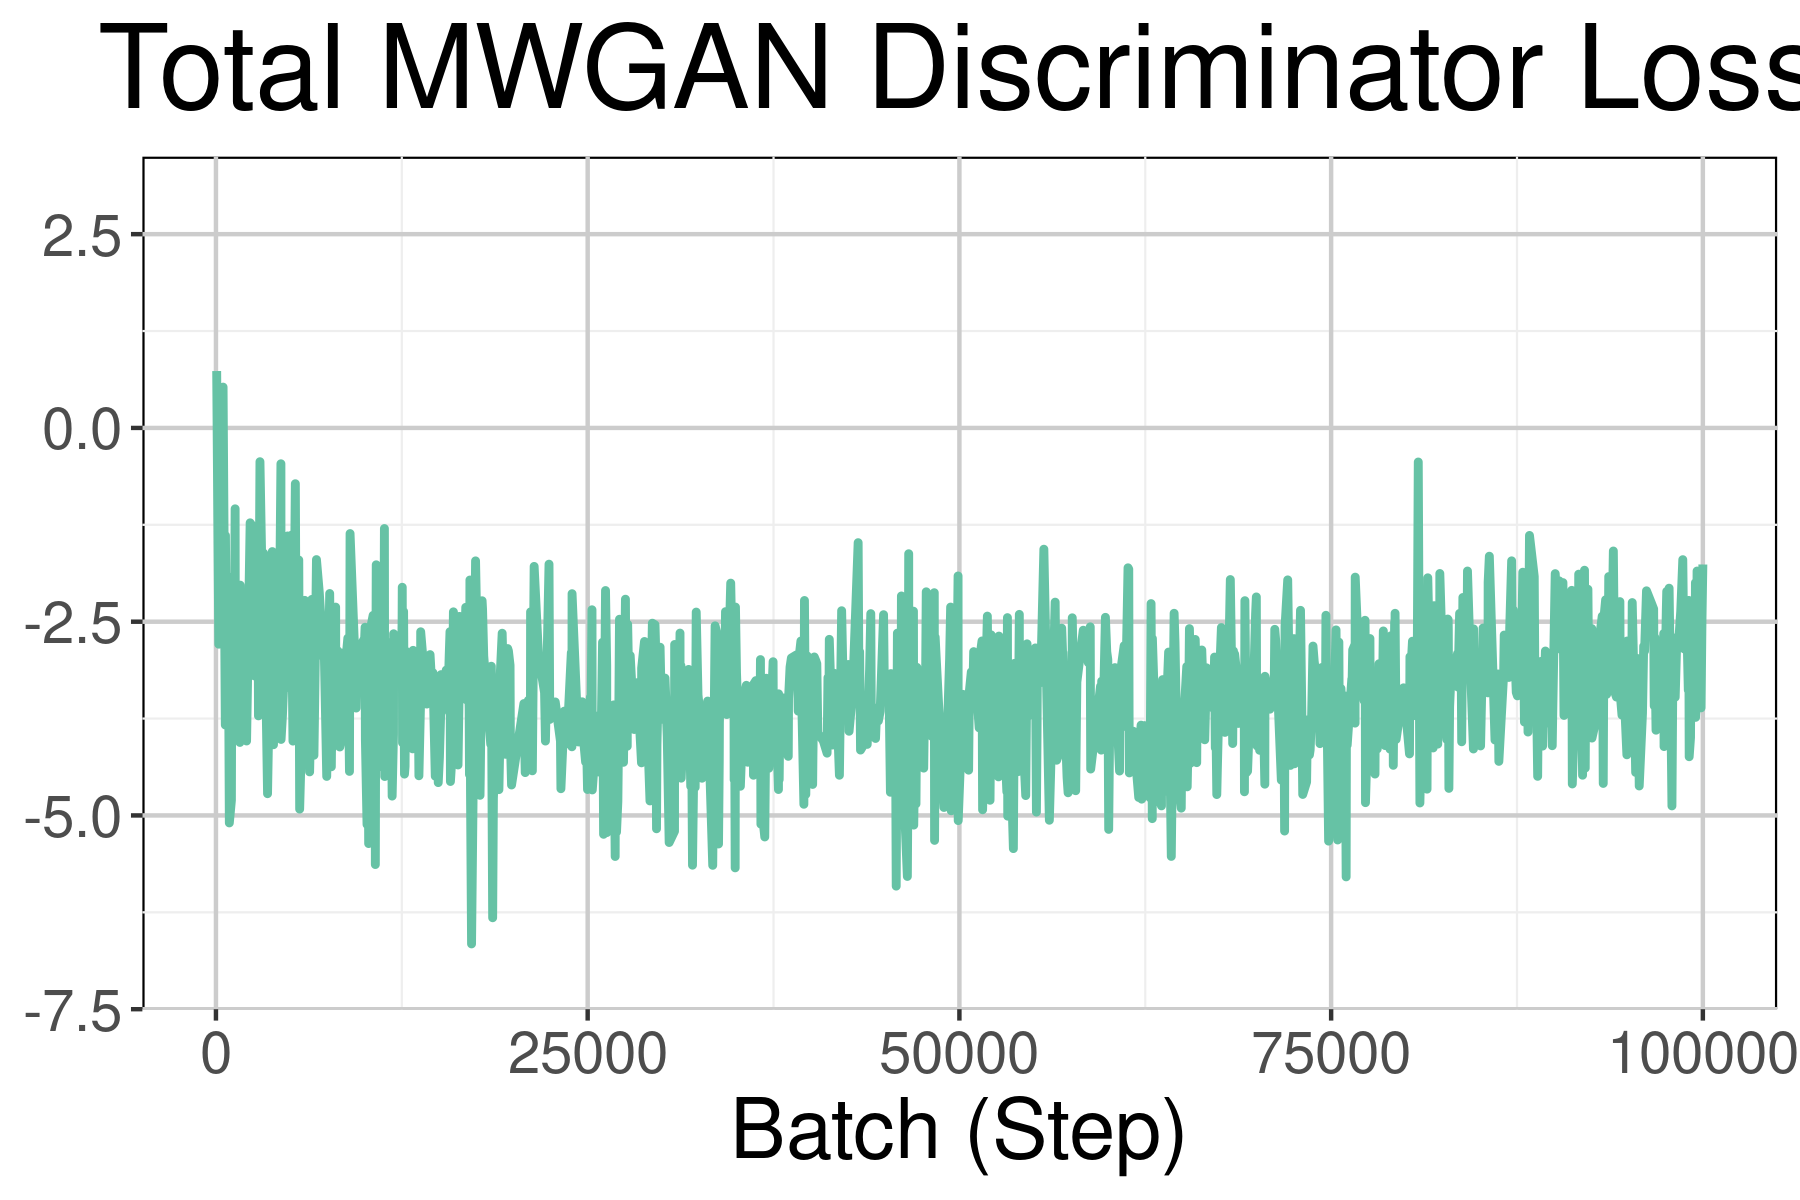
\includegraphics[width=0.45\textwidth]{6_demd/figs/mwgan_disc_convergence.png}
    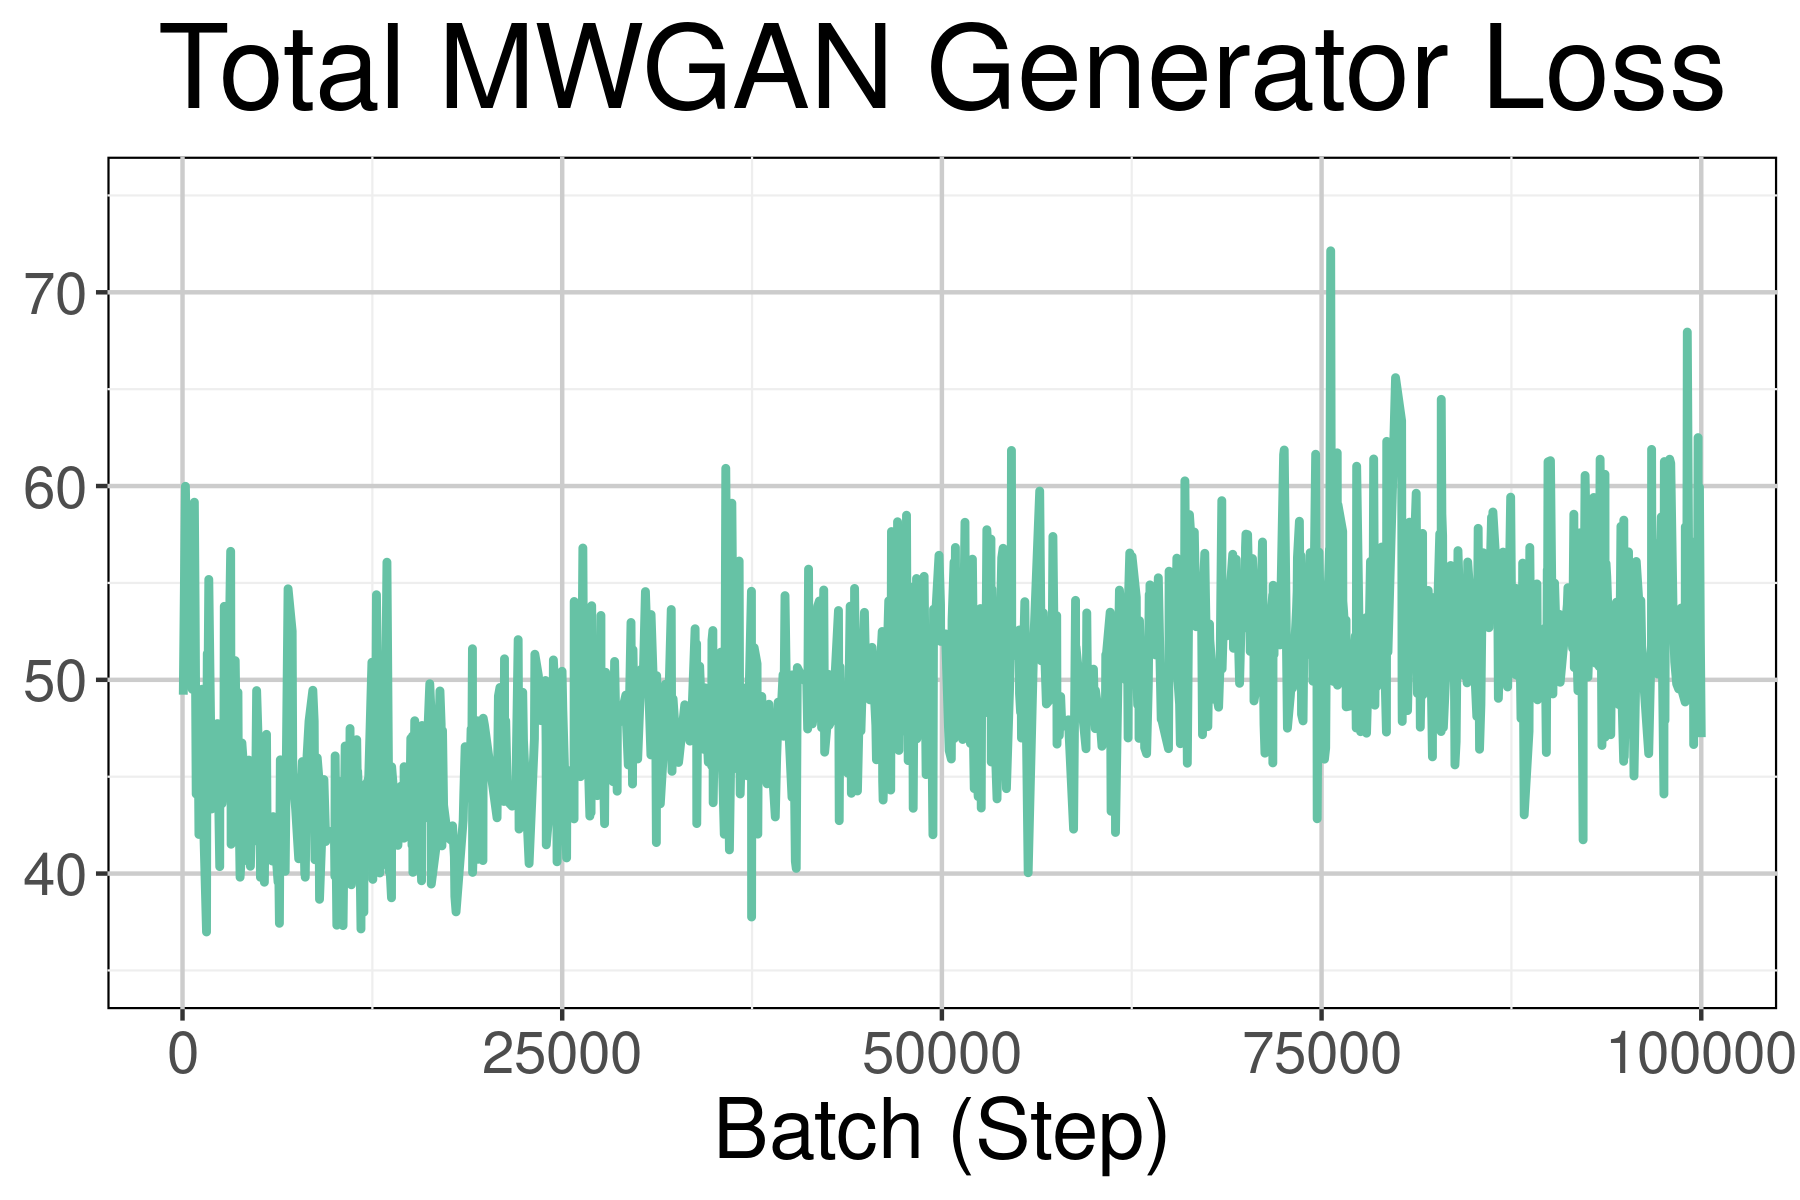
\includegraphics[width=0.45\textwidth]{6_demd/figs/mwgan_gen_convergence.png}
    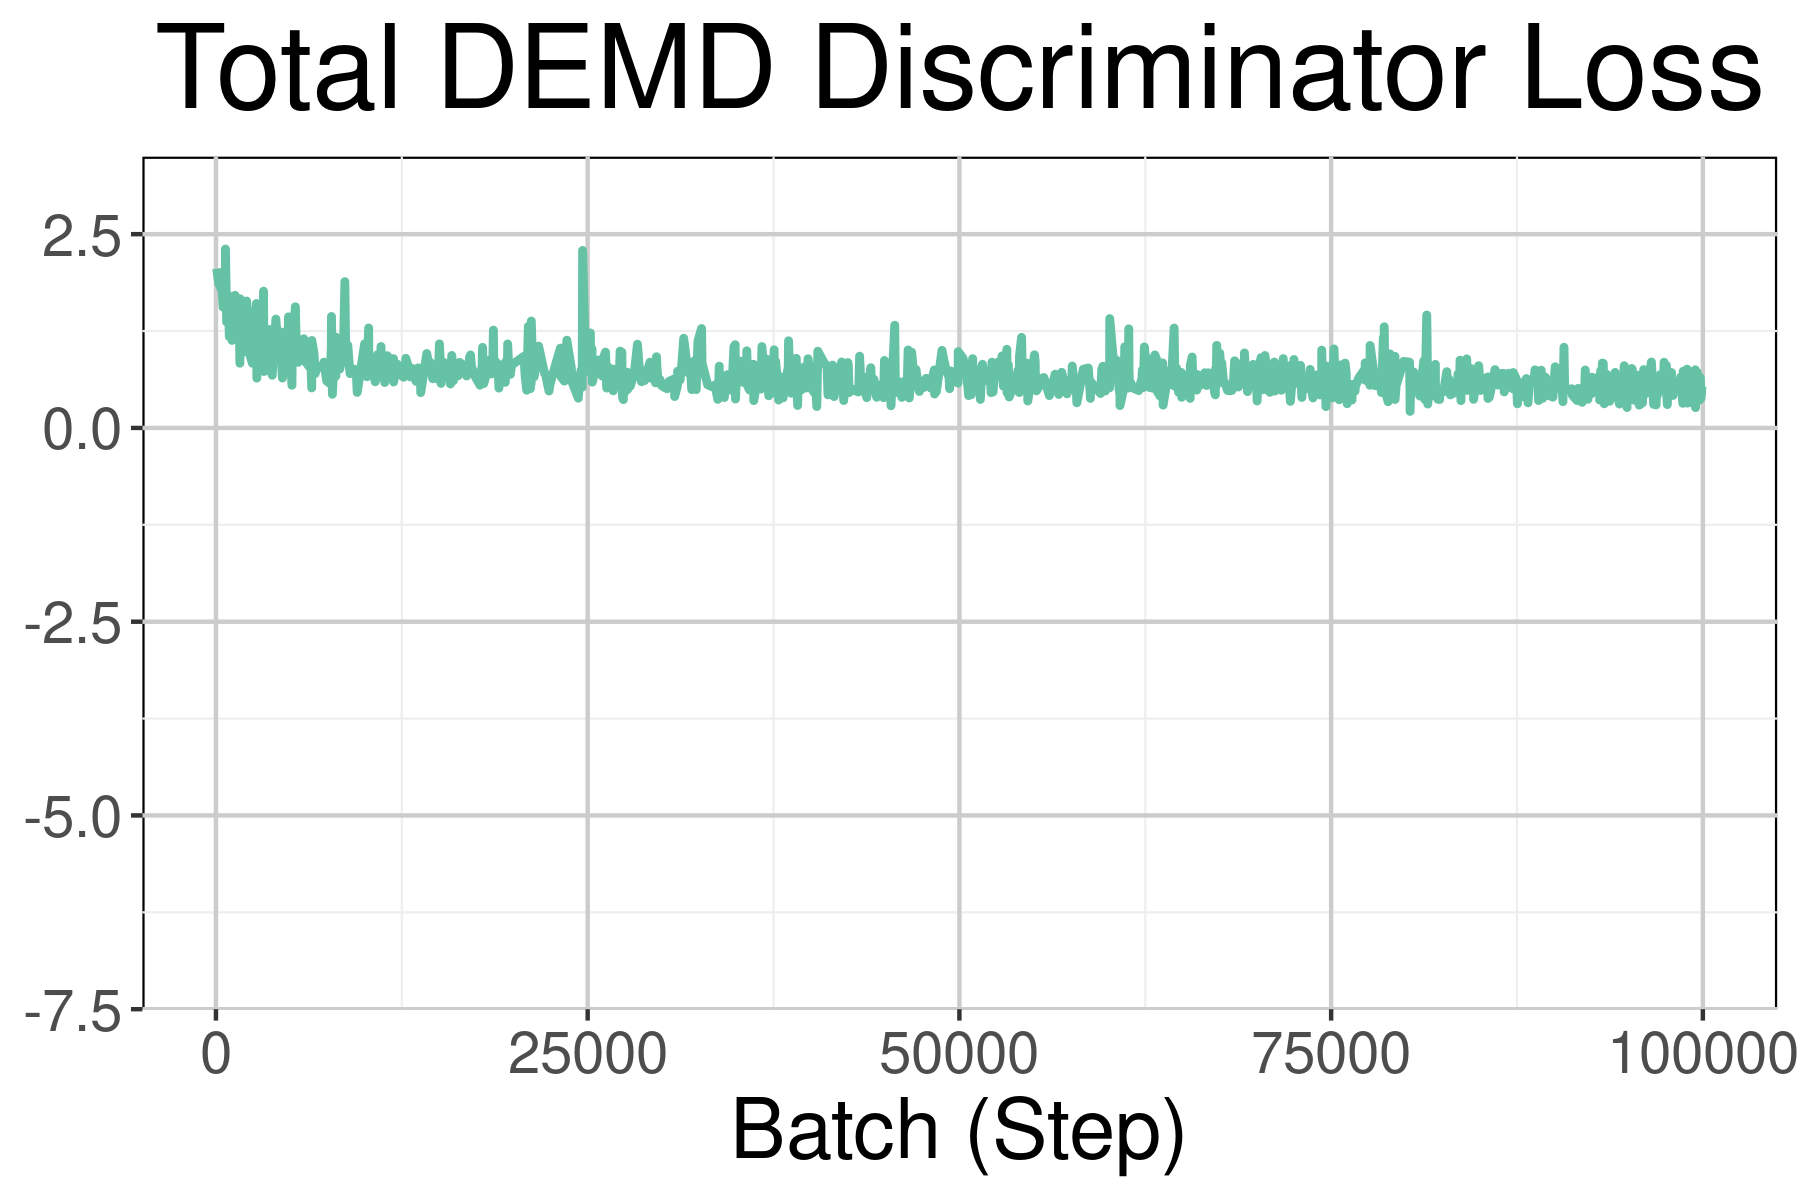
\includegraphics[width=0.45\textwidth]{6_demd/figs/demd_disc_convergence.png}
    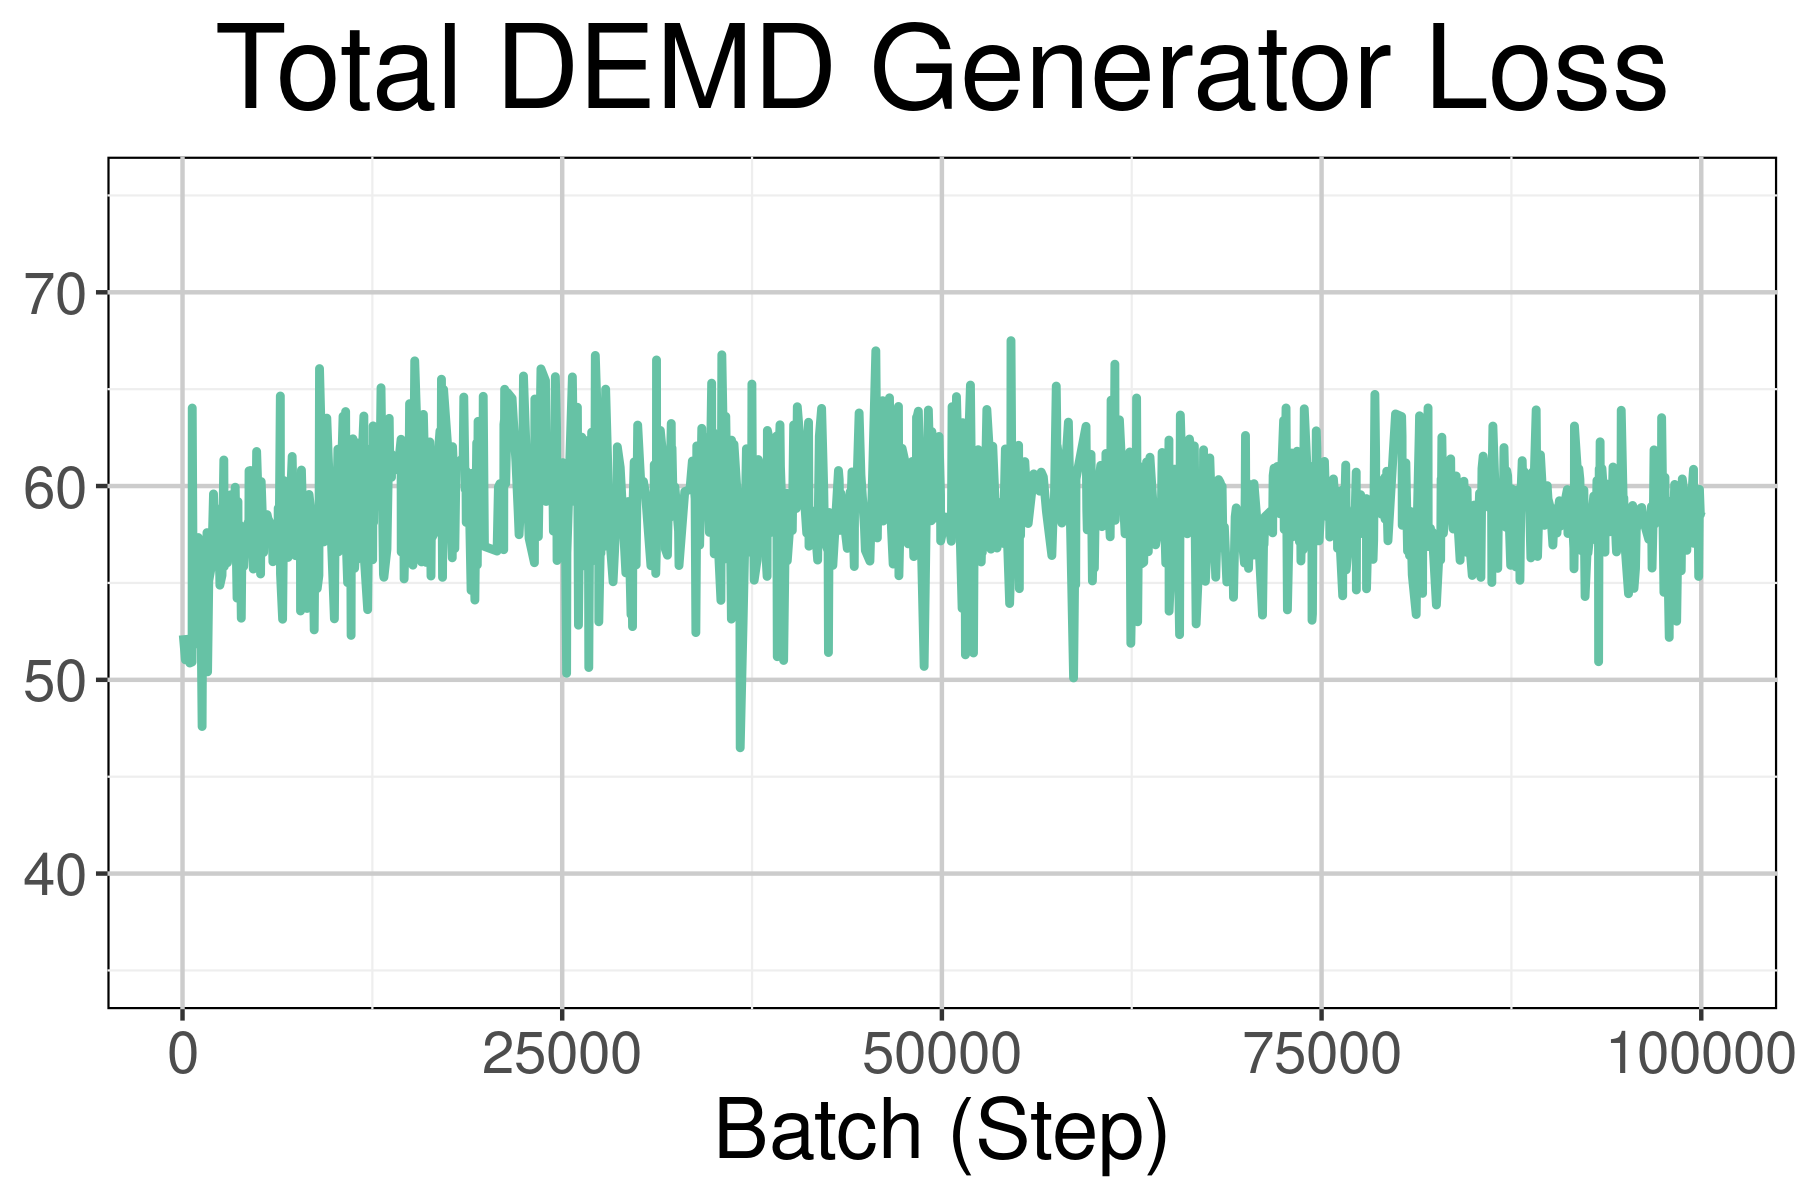
\includegraphics[width=0.45\textwidth]{6_demd/figs/demd_gen_convergence.png}
    \caption{Convergence Plots for MWGAN and DEMD on CelebA Multi-Domain Image Translation.}
    \label{fig:convergence}
\end{figure}

The MWGAN code \url{https://github.com/deepmo24/MWGAN} was used under the MIT license extended from the original StarGAN codebase \url{https://github.com/yunjey/stargan}.

The original paper constructs an inter-domain penalty added to the multi-domain GAN discriminator loss as follows:
\
\begin{align}
    R_{MWGAN} (f) = \lambda \cdot \left( \sum_i \EE_{\tilde{x}^{(i)}\sim \hat{\QQ}_i} ||\nabla f(\tilde{x}^{(i)})|| - L_f\right)^2_{+}
\end{align}
The sampling for expectation in practice is done by interpolating randomly between real data and generated data for each domain. In contrast to this, we directly push the gradient norms computed over samples from each domain to be close using our DEMD regularizer:
\begin{align}
    R_{DEMD} (f) = \lambda \cdot DEMD\left( \left[||\nabla f(\tilde{x}^{(i)})||\right]_i , [i] \right),
\end{align}
where $[i]$ indicates the domain associated with the fake samples generated in the same manner for each domain.

\paragraph{Convergence Comparison.}
Interestingly we observe that our construction tends to lead to more stable training. In Figure~\ref{fig:convergence}, we can see that the variance of the total discriminator and generator loss fluctuate much less. We suspect that this can be directly attributed to the boundedness of the gradients of the DEMD regularizer, specific to the method where we compute the gradients via the dual of the LP: the dual variables are bounded by definition and in this particular LP, are bounded exactly by the number of bins used for discretization. While additional investigation is needed, smoothness has been identified as a desirable property of GAN training \citep{pmlr-v70-arora17a,Chu2020Smoothness}.

\paragraph{Quantitative Results.}
Using the Frechet Inception Distance we quantitatively measure the resulting generative samples. Following the description in \cite{cao2019multi}, we present the FID scores of our model and theirs in Table~\ref{tab:fidtrain}. Our metric as a drop-in replacement performs comparably.

\begin{table}
    \centering
    \begin{tabular}{l|c|c|c|c}
        \toprule
        Model & Blond Hair & Eyeglasses & Mustache & Pale Skin \\
        \midrule
        MWGAN~\cite{cao2019multi} & 49.91 & 45.74 & 45.49 & 38.67 \\
        DEMD & 47.29 & 34.43 & 50.69 & 39.60 \\
        \bottomrule
    \end{tabular}
    \caption[Caption for LOF]{Train FID Scores for CelebA Multi-Domain Image Translation.\protect\footnotemark}
    \label{tab:fidtrain}
\end{table}
\footnotetext{Results presented here computed using the pytorch-fid package with code from the MWGAN repository here: \url{https://github.com/mseitzer/pytorch-fid}. We were unable to replicate the FID scores provided in the original paper, but expect trends to be relatively similar when compared across different scoring methods.}

% \begin{table}[]
%     \centering
%     \begin{tabular}{l|c|c|c|c}
%         \toprule
%         Model & Blond Hair & Eyeglasses & Mustache & Pale Skin \\
%         \midrule
%         MWGAN~\cite{cao2019multi} & 90.85 & 115.90 & 127.29 & 120.89 \\
%         DEMD & 94.45 & 95.52 & 129.79 & 114.95 \\
%         \bottomrule
%     \end{tabular}
%     \caption[Caption for LOF]{Test FID Scores for CelebA Multi-Domain Image Translation.\protect\footnotemark}
%     \label{tab:fidtest}
% \end{table}

\begin{figure}
    \centering
    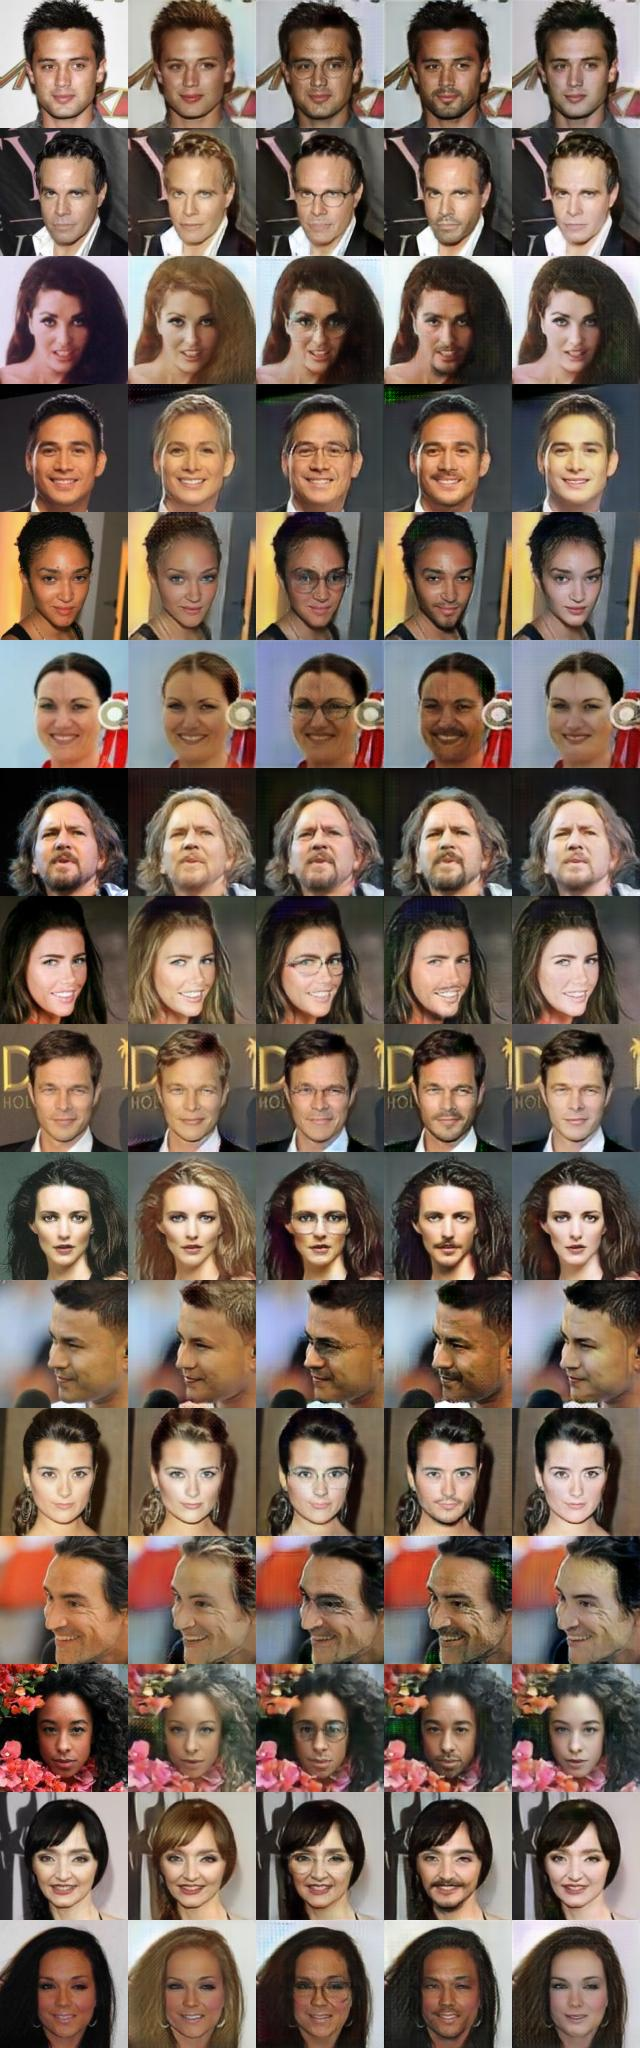
\includegraphics[height=0.85\textheight]{6_demd/figs/mwgan_res/mwgan-00001-images.jpg}
    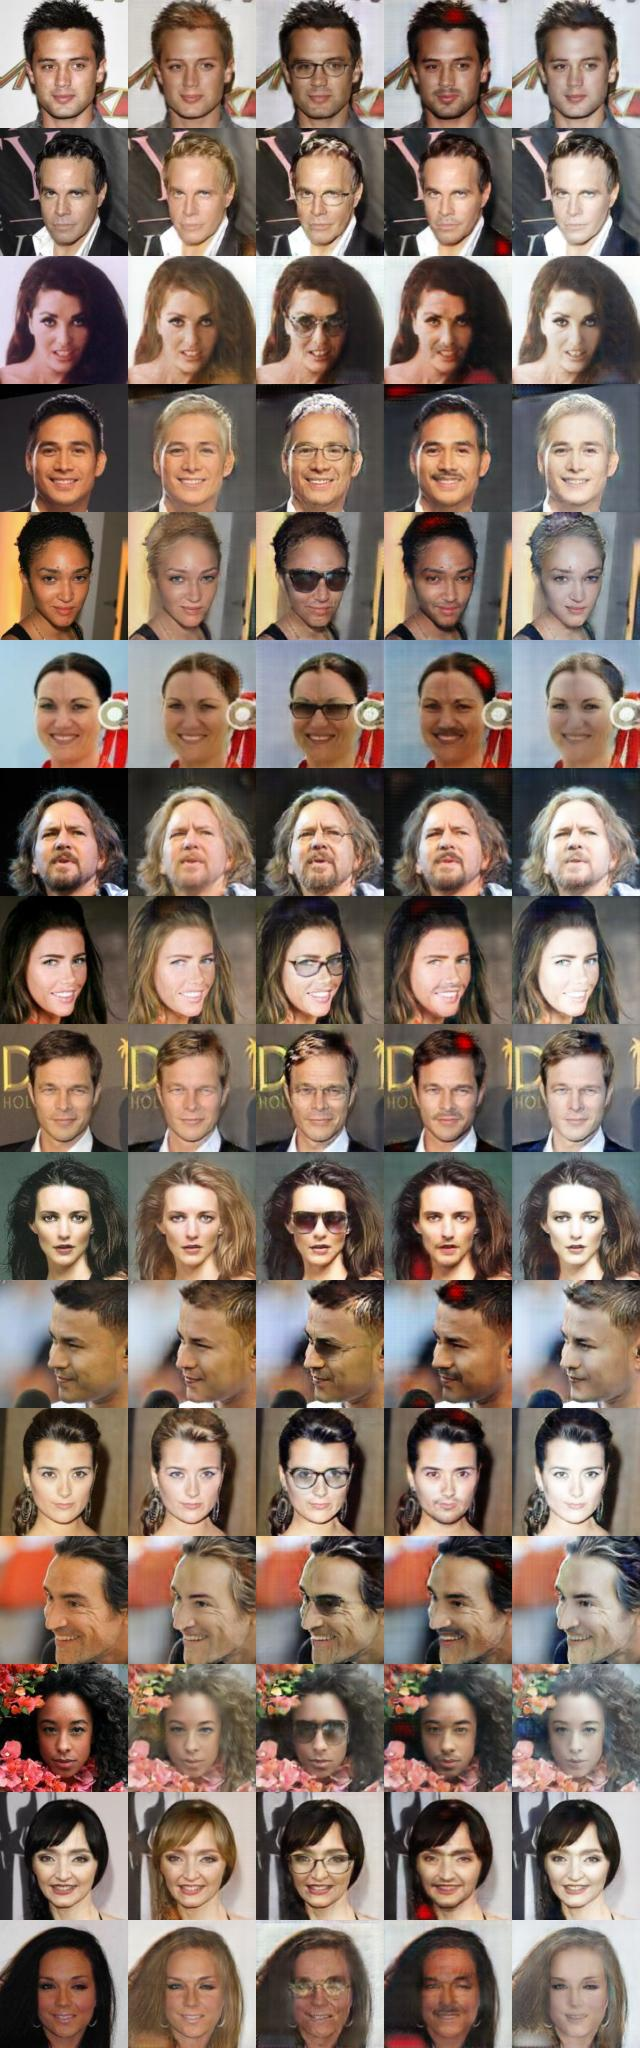
\includegraphics[height=0.85\textheight]{6_demd/figs/mwgan_res/demd-00001-images.jpg}
    \caption{More qualitative results from the multi-domain image translation problem with (Left) \cite{cao2019multi}, (Right) DEMD (ours). On attributes such as ``Blond Hair'' and ``Eyeglasses'', the generated images through our DEMD procedure appear more realistic. On other attributes, the generated images are comparable. }
    \label{fig:moreganres1}
\end{figure}

\begin{figure}
    \centering
    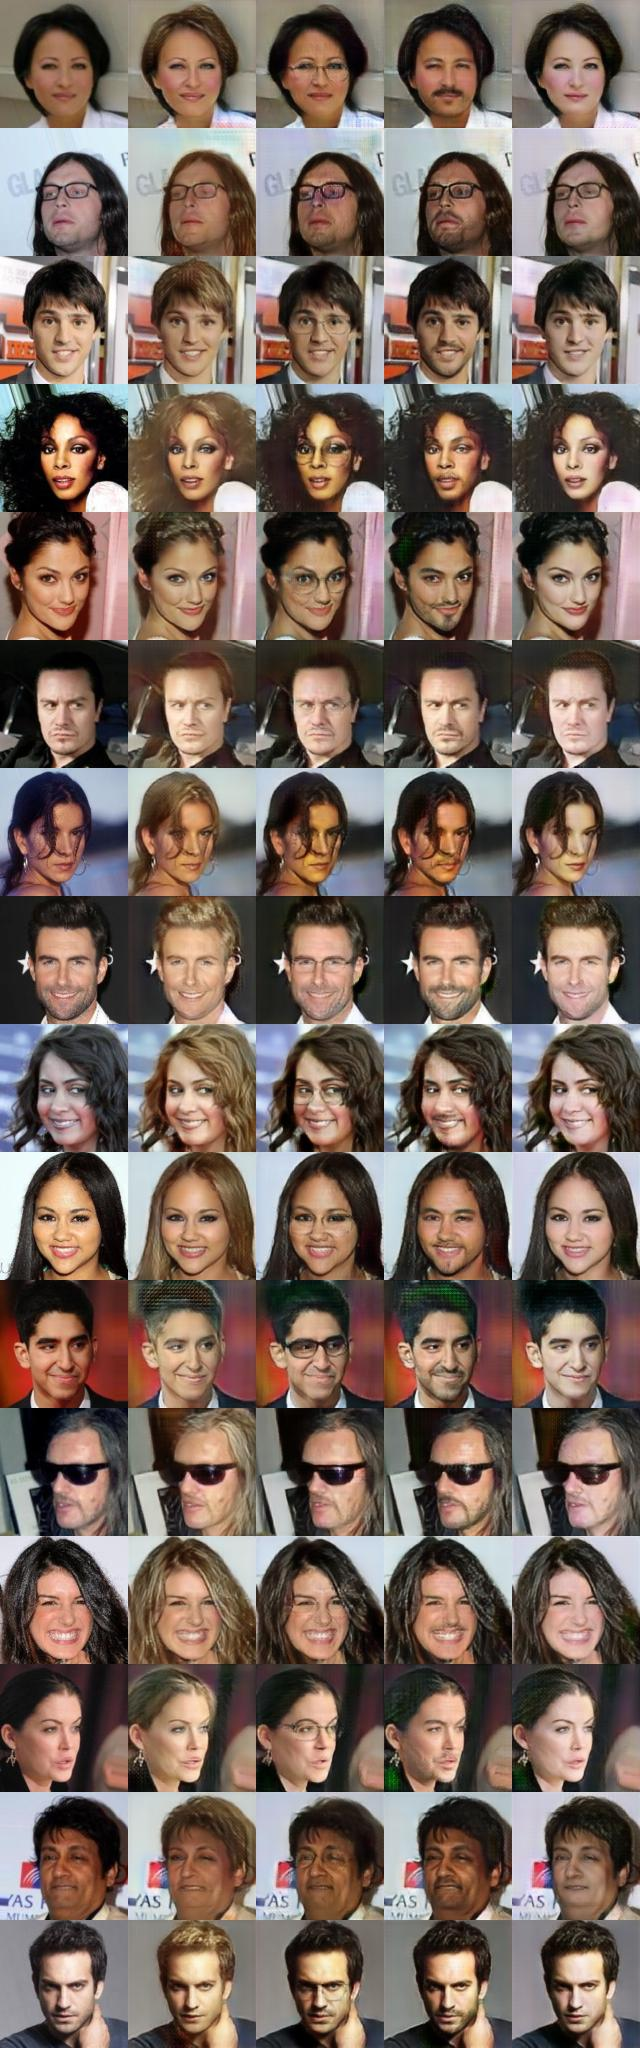
\includegraphics[height=0.85\textheight]{6_demd/figs/mwgan_res/mwgan-00003-images.jpg}
    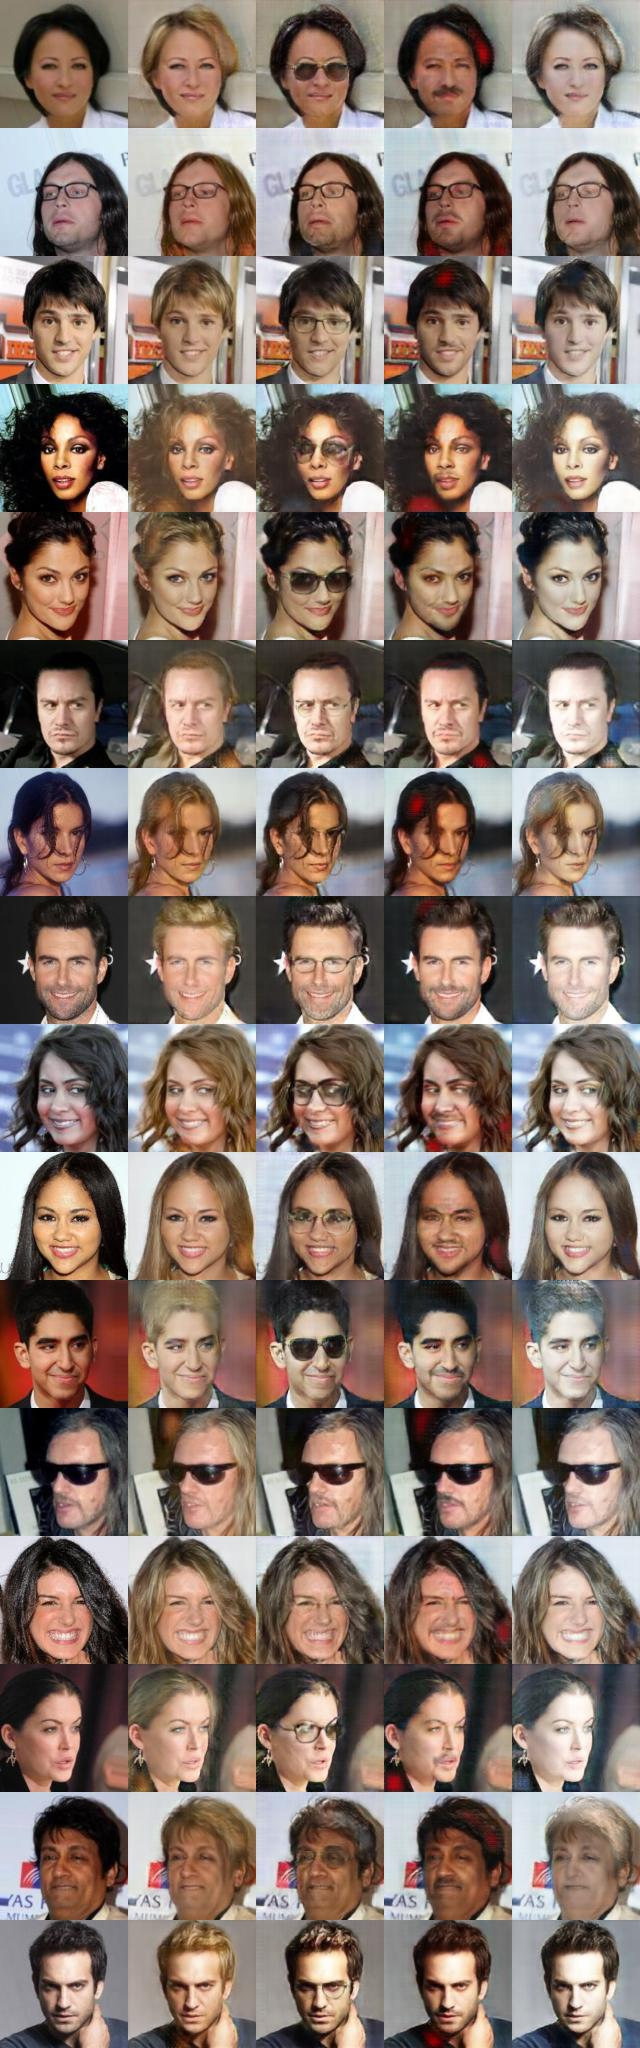
\includegraphics[height=0.85\textheight]{6_demd/figs/mwgan_res/demd-00003-images.jpg}
    \caption{More qualitative results from the multi-domain image translaton problem with (Left) \cite{cao2019multi}, (Right) DEMD (ours). On attributes such as ``Blond Hair'' and ``Eyeglasses'', the generated images through our DEMD procedure appear more realistic. On other attributes the generated images are comparable. }
    \label{fig:moreganres2}
\end{figure}